\begin{frame}
  \frametitle{Classifying images}

  \begin{center}
    Classification is an \textit{supervised} learning task by which we
    aim to predict the correct label for an example given its features
    \vskip20pt

    \only<1>{
    
\includegraphics[width=0.5\textwidth]{ocr.png} \\
    \Huge{$\downarrow$} \\
    \Huge{0 \hskip10pt 5 \hskip10pt 4 \hskip10pt 1 \hskip10pt 4 \hskip10pt 9}
    \vskip20pt
    \normalsize
    e.g. determine which digit $\{0,1,\ldots,9\}$ is in depicted in each image
    }

    \only<2>{
      \begin{tabular}{cc}
        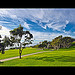
\includegraphics[height=0.2\textheight]{landscape.jpg} & 
\includegraphics[height=0.2\textheight]{headshot.jpg} \\
        $\downarrow$ & $\downarrow$ \\
        'landscape' & 'headshot'
      \end{tabular}
    \vskip20pt
    \normalsize
    e.g. determine if an image is a landscape or headshot
    }

  \end{center}

\end{frame}


\begin{frame}
  \frametitle{k-nearest neighbors classification}

  \begin{center}
    k-nearest neighbors: memorize training examples, predict labels using labels of the k closest training points
    \vskip20pt
    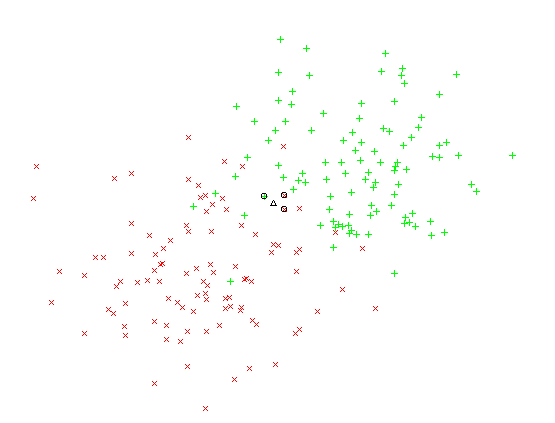
\includegraphics[width=0.65\textwidth]{knn_schematic.png}
    \vskip10pt
    Intuition: nearby points have similar labels
  \end{center}

\end{frame}


\begin{frame}
  \frametitle{k-nearest neighbors classification}

  \begin{center}
    %\vskip20pt
    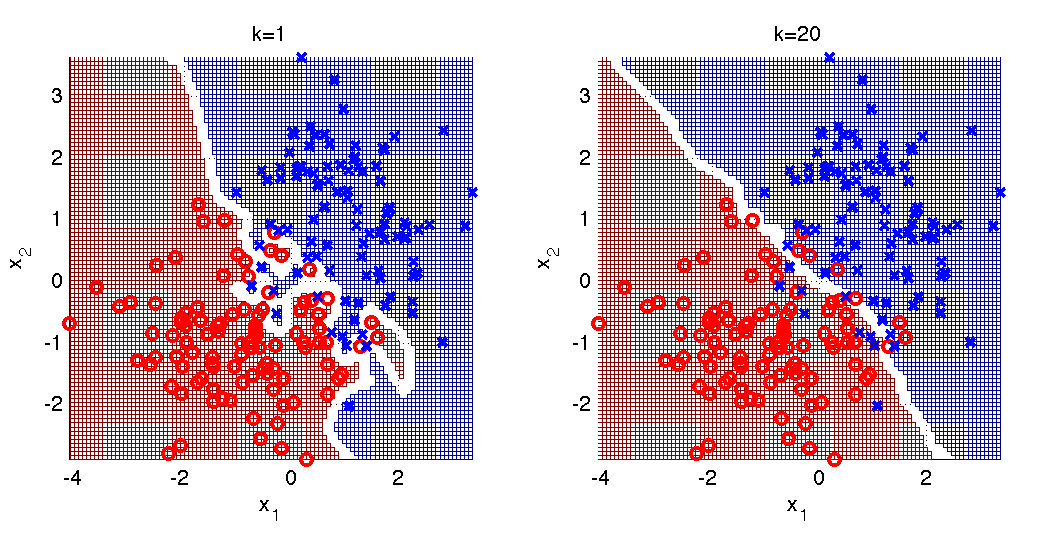
\includegraphics[width=\textwidth]{knn_boundary.png}
    \vskip10pt
    \textbf{Small k} gives a \textbf{complex} boundary, \textbf{large
      k} results in \textbf{coarse} averaging
  \end{center}

\end{frame}

\begin{frame}[fragile]
  \frametitle{k-nearest neighbors classification}

  \begin{center}
    \begin{block}{A simple kNN implementation with SciPy}
        \begin{lstlisting}[language=python]
import scipy.spatial as spat

# use the cdist function to quickly compute distances
# between all test and training examples
D = spat.distance.cdist(X, self.X, 'euclidean')

for i in range(N):
    # grab the indices of the k closest points
    ndx = D[i,:].argsort()[:k]

    # take a majority vote over the nearest points'
    # labels
    yhat[i] = mode(self.y[ndx])[0]
        \end{lstlisting}
    \end{block}
  \end{center}
\end{frame}


\begin{frame}
  \frametitle{Digit recognition}

  \begin{center}
    Determine which digit $\{0,1,\ldots,9\}$ is in depicted in each image
    \vskip10pt
    
\includegraphics[width=0.65\textwidth]{../../code/image_data/sample_digits.png}
    %
\includegraphics[width=0.5\textwidth]{ocr.png} \\
    %\Huge{$\downarrow$} \\
    %\Huge{0 \hskip10pt 5 \hskip10pt 4 \hskip10pt 1 \hskip10pt 4 \hskip10pt 9}
    %\vskip20pt
    %\normalsize
    \vskip10pt
    Represent each image as a ``bag of pixels'', flattening the 2-d array
    of pixels to a 1-d vector

  \end{center}
\end{frame}


\begin{frame}[fragile]
  \frametitle{Digit recognition}

  \begin{center}
    \begin{block}{Simple digit classifer with k=1 nearest neighbors}
        \begin{lstlisting}[language=bash]
 ./classify_digits.py
        \end{lstlisting}
    \end{block}
    \vskip20pt
    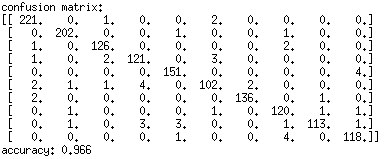
\includegraphics[width=0.55\textwidth]{digits_confmat.png}
  \end{center}
\end{frame}



\begin{frame}
  \frametitle{Image classification}

  \begin{center}
    Determine if an image is a landscape or headshot
    \vskip20pt
      \begin{tabular}{cc}
        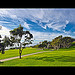
\includegraphics[height=0.2\textheight]{landscape.jpg} & 
\includegraphics[height=0.2\textheight]{headshot.jpg} \\
        $\downarrow$ & $\downarrow$ \\
        'landscape' & 'headshot'
      \end{tabular}
    \vskip20pt
    Represent each image with a binned RGB intensity histogram

  \end{center}
\end{frame}


\begin{frame}[fragile]
  \frametitle{Image classification}

  \begin{center}
    \begin{block}{Classify}
        \begin{lstlisting}[language=bash]
 ./classify_flickr.py 16 9 
    flickr_headshot flickr_landscape
        \end{lstlisting}
    \end{block}
    \vskip20pt
    \begin{block}{Change in performance with number of neighbors}
        \begin{lstlisting}[language=bash]
k = 1, accuracy = 0.7125
k = 3, accuracy = 0.7425
k = 5, accuracy = 0.7725
k = 7, accuracy = 0.7650
k = 9, accuracy = 0.7500
        \end{lstlisting}
    \end{block}
    %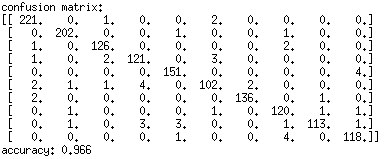
\includegraphics[width=0.55\textwidth]{digits_confmat.png}
  \end{center}
\end{frame}
